% Latex template: mahmoud.s.fahmy@students.kasralainy.edu.eg
% For more details: https://www.sharelatex.com/learn/Beamer

\documentclass{beamer}					% Document class
\geometry{papersize={15cm,10cm}}

%\setbeamertemplate{footline}[text line]{%
%  \parbox{\linewidth}{\vspace*{-8pt}\hfill\hfill\insertpagenumber}}
\setbeamertemplate{navigation symbols}{}

\usepackage[english]{babel}				% Set language
\usepackage[utf8x]{inputenc}			% Set encoding

\mode<presentation>						% Set options
{
  \usetheme{default}					% Set theme
  \usecolortheme{default} 				% Set colors
  \usefonttheme{default}  				% Set font theme
  \setbeamertemplate{caption}[numbered]	% Set caption to be numbered
}

% Uncomment this to have the outline at the beginning of each section highlighted.
%\AtBeginSection[]
%{
%  \begin{frame}{Outline}
%    \tableofcontents[currentsection]
%  \end{frame}
\usepackage{graphicx}					% For including figures
\usepackage{booktabs}					% For table rules
\usepackage{hyperref}	
\usepackage{tikz-network}				% For cross-referencing
\usepackage[absolute,overlay]{textpos}
\usepackage{bm}
\usepackage[font=small,labelfont=bf]{caption}				% For cross-referencing
\usepackage{comment}
\usepackage{braket}
\usepackage{animate}

\title{Imaging and analysis strategies in the era of spatial omics}	% Presentation title
\author{Clayton W. Seitz, Ph.D.}								% Presentation author
\date{\today}									% Today's date	

\AtBeginSection[]{
  \begin{frame}
  \vfill
  \centering
  \begin{beamercolorbox}[sep=8pt,center,shadow=true,rounded=true]{title}
    \usebeamerfont{title}\insertsectionhead\par%
  \end{beamercolorbox}
  \vfill
  \end{frame}
}

\begin{document}

% Title page
% This page includes the informations defined earlier including title, author/s, affiliation/s and the date
\begin{frame}
  \titlepage
\end{frame}

\begin{frame}{About Me}

\begin{textblock*}{10cm}(1.0cm,3cm)
\textbf{Education}
\begin{itemize}
\item PhD @ Purdue University, MS @ University of Chicago
\end{itemize}
\end{textblock*}

\begin{textblock*}{10cm}(1.0cm,5cm)
\textbf{Research interests}
\begin{itemize}
\item Bioimaging, Machine learning methods for live cell imaging
\item Quantitative single molecule localization microscopy 
\item Generative models, statistical physics, theory of deep learning
\end{itemize}
\end{textblock*}

\end{frame}

\begin{frame}{Outline of the talk}
    \tableofcontents
\end{frame}



% The following is the most frequently used slide types in beamer
% The slide structure is as follows:
%
%\begin{frame}{<slide-title>}
%	<content>
%\end{frame}

\setbeamertemplate{footline}{
    \hbox{%
    \begin{beamercolorbox}[wd=\paperwidth,ht=1.0ex,dp=1.5ex,leftskip=2ex,rightskip=2ex]{page ooter}%
        \footnotesize
        \usebeamerfont{title in head/foot}%
        Introduction to fluorescence nanoscopy \hfill
            %\insertsection \hfill
        \insertframenumber{} / \inserttotalframenumber
    \end{beamercolorbox}}%
}


\section{Motivation for spatial biology}

\section{Localization microscopy for spatial biology}


\begin{frame}{Single molecule localization microscopy}
\begin{textblock*}{9cm}(0.5cm,1.5cm)
\includegraphics[width=\textwidth]{../../phd/dissertation/dissertation/media/Intro-Cropped.png}
\end{textblock*}
\begin{textblock*}{5cm}(9.5cm,1.5cm)
\animategraphics[width=5cm,autoplay,loop]{60}{../../phd/dissertation/dissertation/media/storm-animation/storm-animation-}{1}{100}
\end{textblock*}
\begin{textblock*}{15cm}(0.5cm,7.5cm)
\begin{itemize}
\item STORM and similar nanoscopy techniques are limited by localization precision
\item Higher lateral/axial resolution than other methods (e.g., SIM,STED,Confocal)
\item Poor time resolution
\end{itemize}
\end{textblock*}
\end{frame}

\begin{frame}{Stochastic optical reconstruction microscopy (STORM)}
\begin{textblock*}{9cm}(0.5cm,1.5cm)
\includegraphics[width=\textwidth]{../../phd/dissertation/dissertation/media/Intro-Cropped.png}
\end{textblock*}
\begin{textblock*}{5cm}(9.5cm,1.5cm)
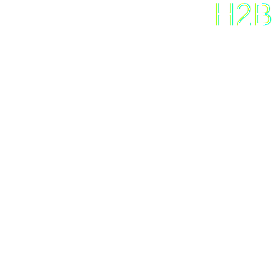
\includegraphics[width=\textwidth]{../../phd/dissertation/dissertation/media/STORM-Example.png}
\end{textblock*}
\begin{textblock*}{15cm}(0.5cm,7.5cm)
\begin{itemize}
\item STORM and similar nanoscopy techniques are limited by localization precision
\item Higher lateral/axial resolution than other methods (e.g., SIM,STED,Confocal)
\item Poor time resolution
\end{itemize}
\end{textblock*}
\end{frame}

\begin{frame}{Nanoscopy by localizing isolated fluorescent emitters}
\begin{itemize}
\item Modeling the point spread function permits sub-pixel localization 
\end{itemize}
\begin{textblock*}{8cm}(6.5cm,3.0cm)
\includegraphics[width=\textwidth]{../../phd/dissertation/dissertation/media/Model.png}
\end{textblock*}

\begin{textblock*}{2cm}(1cm,2.0cm)
\begin{align*}
\mu_{k} &= i_{0}\int\int O(u,v)dudv + \textcolor{pink}{\lambda}\\
i_{0} &= g_{k}\textcolor{red}{\eta} \textcolor{cyan}{\zeta}\textcolor{blue}{\Delta} 
\\
g_{k} &- \mathrm{pixel\; gain}\\
\textcolor{red}{\eta} &- \mathrm{quantum\; efficiency}\\
\textcolor{cyan}{\zeta} &- \mathrm{photon\; emission\; rate}\\
\textcolor{blue}{\Delta} &- \mathrm{exposure\; time}\\
\textcolor{pink}{\lambda} &- \mathrm{background \; rate}
\end{align*}
\end{textblock*}

\vspace{2in}

Maximum likelihood localization:

\begin{equation*}
\theta^{*} = \underset{\theta}{\mathrm{argmax}}\prod_{k}p(\bold{x}_{k}|\theta)= \underset{\theta}{\mathrm{argmin}}-\sum_{k}\log p(\bold{x}_{k}|\theta)
\end{equation*}

\end{frame}



\begin{frame}{Tracking chromatin loci with photoactivated localization microscopy}
\begin{textblock*}{12cm}(1.0cm,1.5cm)
\includegraphics[width=12cm]{../../postdoc/sartorius/media/DOE.png}
Locatelli, Seitz et al. PNAS \textbf{29} (2022)
\end{textblock*}
\begin{textblock*}{14cm}(1.0cm,7.5cm)
\begin{itemize}
\item A diffractive optical element (DOE) is used to photoactivate chromatin microdomains
\item Used for understanding the spatial correlations of chromatin diffusion
\end{itemize}
\end{textblock*}
\end{frame}

\begin{frame}{Tracking chromatin loci with photoactivated localization microscopy}
\begin{textblock*}{12cm}(1.0cm,1.5cm)
\includegraphics[width=12cm]{../../postdoc/sartorius/media/Bleo.png}
Locatelli, Seitz et al. PNAS \textbf{29} (2022)
\end{textblock*}
\end{frame}


\begin{frame}{Analyzing the structure of nucleosome nanodomains with SMLM}
\begin{textblock*}{10cm}(2.0cm,1.5cm)
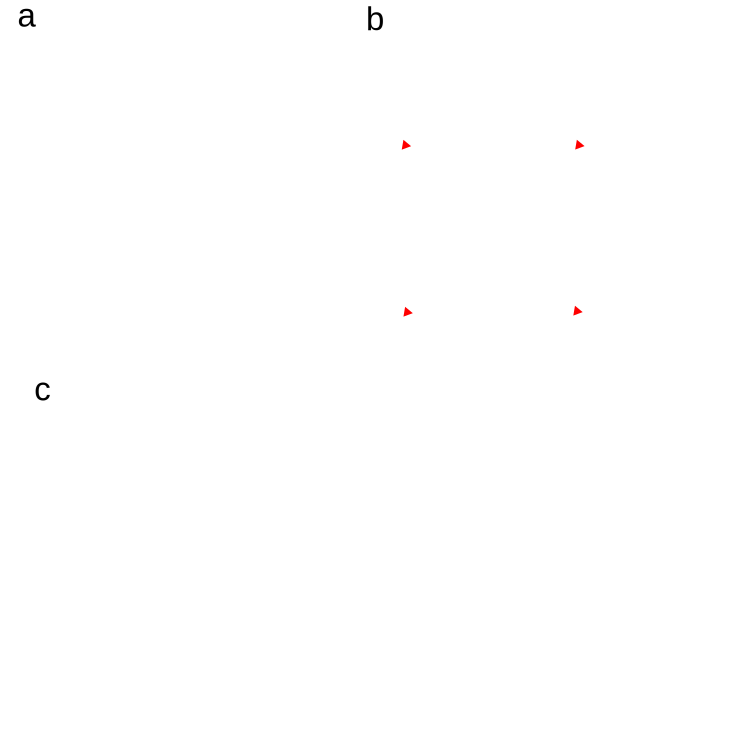
\includegraphics[width=10cm]{../../phd/brd4/brd4/media/Figure-2.png}
Seitz et al. bioRxiv, Cells, In Review (2025)
\end{textblock*}

\begin{textblock*}{13cm}(1.0cm,8.5cm)
\begin{itemize}
\item H2B is densely labeled for super-resolution imaging
\end{itemize}
\end{textblock*}
\end{frame}

\begin{frame}{Spatial organization of HLA-DMB mRNA in T1D}
\begin{textblock*}{10cm}(2.0cm,1.5cm)
\includegraphics[width=10cm]{../../postdoc/spatial/media/HLA-DMB-2.png}
Seitz et al. bioRxiv, Cells, In Review (2025)
\end{textblock*}

\begin{textblock*}{13cm}(1.0cm,8.5cm)
\begin{itemize}
\item H2B is densely labeled for super-resolution imaging
\end{itemize}
\end{textblock*}
\end{frame}

\begin{frame}{Spatial organization of HLA-DMB mRNA in T1D}
\begin{textblock*}{10cm}(2.0cm,1.5cm)
\includegraphics[width=10cm]{../../postdoc/spatial/media/HLA-DMB.png}
Seitz et al. bioRxiv, Cells, In Review (2025)
\end{textblock*}

\begin{textblock*}{13cm}(1.0cm,8.5cm)
\begin{itemize}
\item H2B is densely labeled for super-resolution imaging
\end{itemize}
\end{textblock*}
\end{frame}

\begin{frame}{Multiplexed single molecule localization microscopy}
\includegraphics[width=10cm]{media/Multiplex.png}
\\Chen et al. Science. \textbf{348} (2015)
\end{frame}

\begin{frame}{Multiplexed single molecule localization microscopy}
\includegraphics[width=10cm]{media/MerFISH.png}
\\Chen et al. Science. \textbf{348} (2015)
\end{frame}

\begin{frame}{Multiplexed single molecule localization microscopy}
\includegraphics[width=10cm]{media/Xenium.png}
Wu et al. Trends in Cell Biology. \textbf{30} (2020)
\end{frame}

\begin{frame}{Multiplexed single molecule localization microscopy}
Xenium data example and postprocessing example
\end{frame}


\setbeamertemplate{footline}{
    \hbox{%
    \begin{beamercolorbox}[wd=\paperwidth,ht=1.0ex,dp=1.5ex,leftskip=2ex,rightskip=2ex]{page ooter}%
        \footnotesize
        \usebeamerfont{title in head/foot}%
        Novel methods: probabilistic modeling approaches to fluorescence nanoscopy \hfill
            %\insertsection \hfill
        \insertframenumber{} / \inserttotalframenumber
    \end{beamercolorbox}}%
}

\section{Modeling and analysis approaches in spatial transcriptomics}


\begin{frame}{Selected Publications}

\begin{itemize}

\item \textbf{C. Seitz}, D. Fu, M. Liu, H. Ma, and J. Liu. \textit{BRD4 phosphorylation regulates the structure of chromatin nanodomains}. In Review. Phys Rev Lett. 2024

\item \textbf{C. Seitz} and J. Liu. \textit{Uncertainty-aware localization microscopy by variational diffusion}. In Progress. 2024

\item \textbf{C. Seitz} and J. Liu. \textit{Quantum enhanced localization microscopy with a single photon avalanche diode array}. In Progress. 2024

\item M. Locatelli\textsuperscript{\textdagger}, J. Lawrimore\textsuperscript{\textdagger}, H. Lin\textsuperscript{\textdagger}, S. Sanaullah, \textbf{C. Seitz}, D. Segall, P. Kefer, S. Moreno Naike, B. Lietz, R. Anderson, J. Holmes, C. Yuan, G. Holzwarth, B. Kerry, J. Liu, K. Bonin, P. Vidi. \textit{DNA damage reduces heterogeneity and coherence of chromatin motions}. PNAS 12 July 2022; 119 (29): 1-11

\item M. Zhang, \textbf{C. Seitz}, G. Chang, F. Iqbal, H. Lin, and J. Liu \textit{A guide for single-particle chromatin tracking in live cell nuclei}. Cell Biology International 15 January 2022; 46 (5): 683-700


\end{itemize}
\end{frame}



\end{document}